\documentclass[10pt,a4paper]{article}
\usepackage[utf8]{inputenc}
\usepackage{amsmath}
\usepackage{amsfonts}
\usepackage{amssymb}
\usepackage{graphicx}
\usepackage{enumerate}
\begin{document}

\section{Set Theory}

To demystify mathematics consider
\begin{enumerate}[(i)]
\item What is a theorem?
\item What is a proof?
\end{enumerate}
What if we don't know the answer?

To begin we need
\begin{enumerate}[(a)]
\item an example(s)
\item a nearly related concept
\end{enumerate}


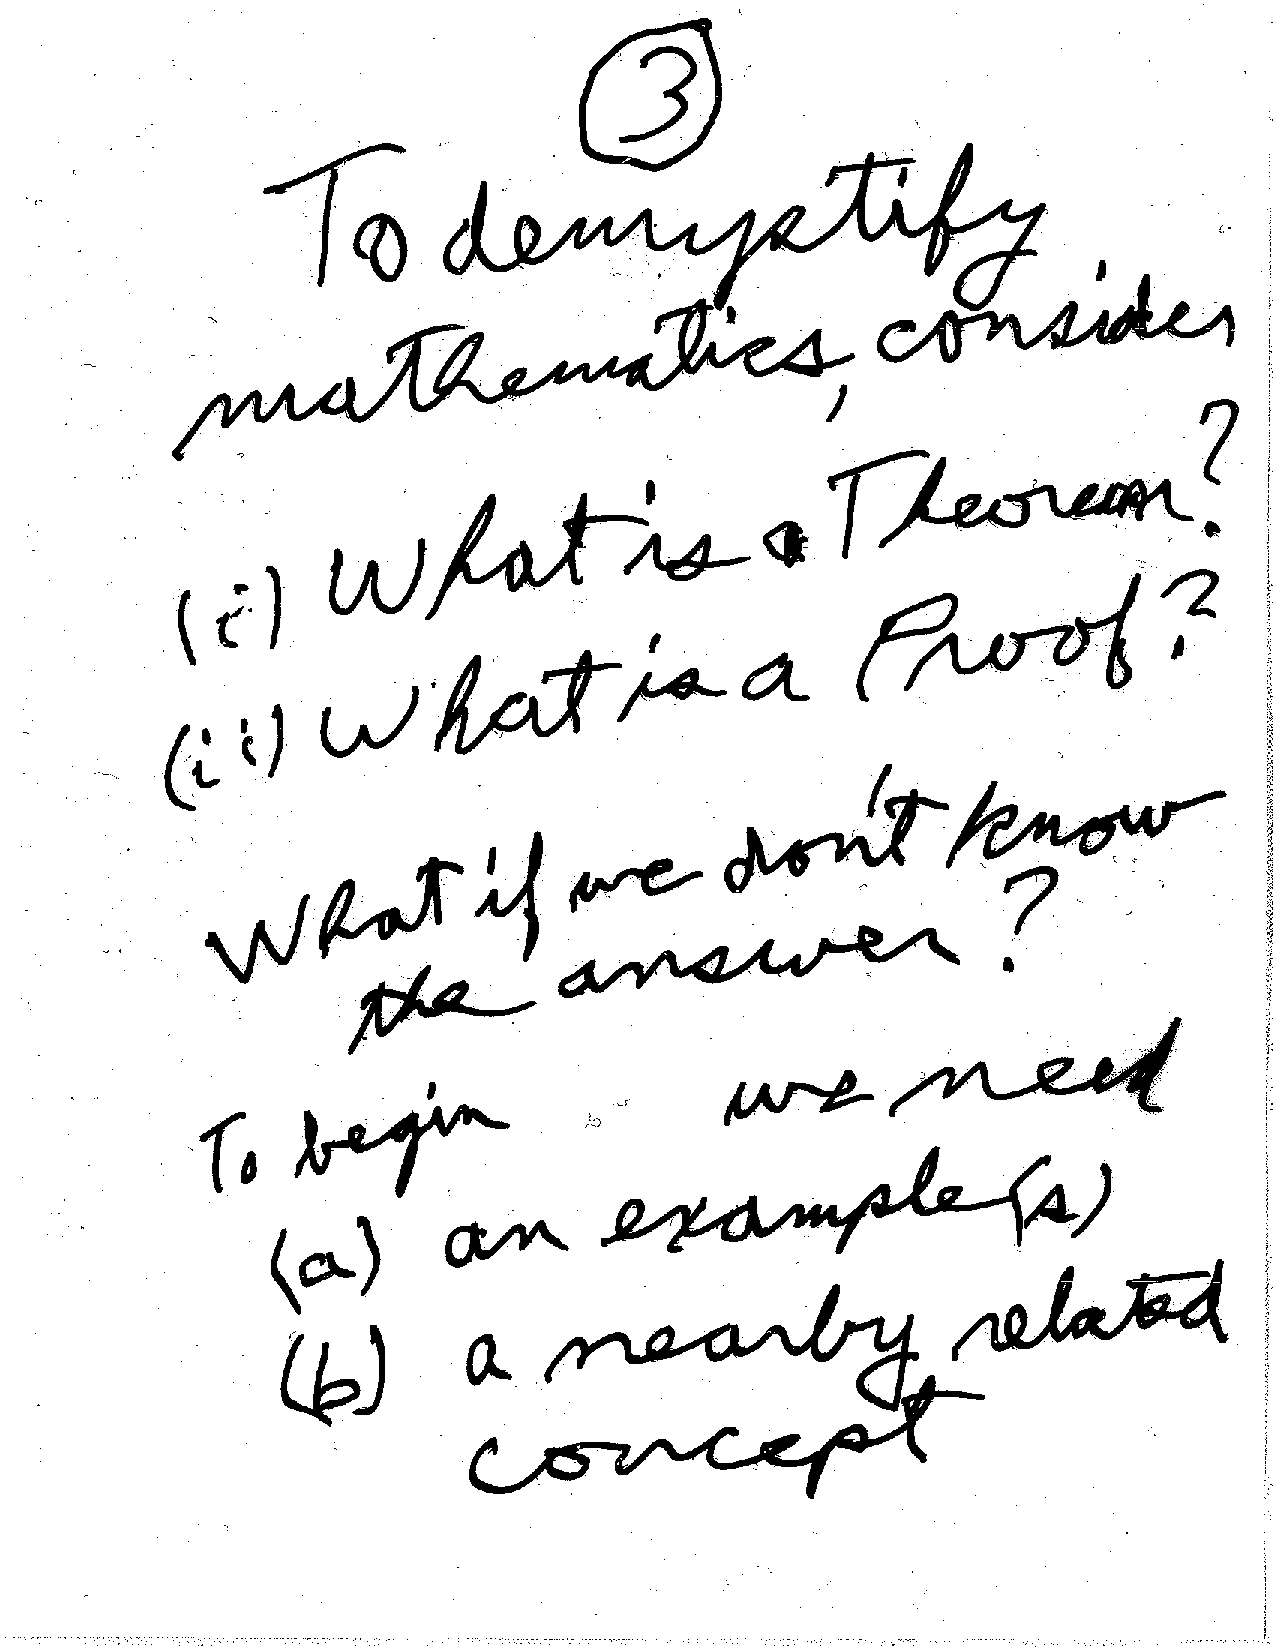
\includegraphics[scale=.5]{Pages/ST_3}

\newpage

Related Concept: Greek Syllogism

\underline{example:}
\begin{enumerate}
\item All men are mortal.
\item Socrates is a man.
\item Therefore, Socrates must die. 
\end{enumerate}

To analyze, recast in set theoretic terms via Venn Diagram.

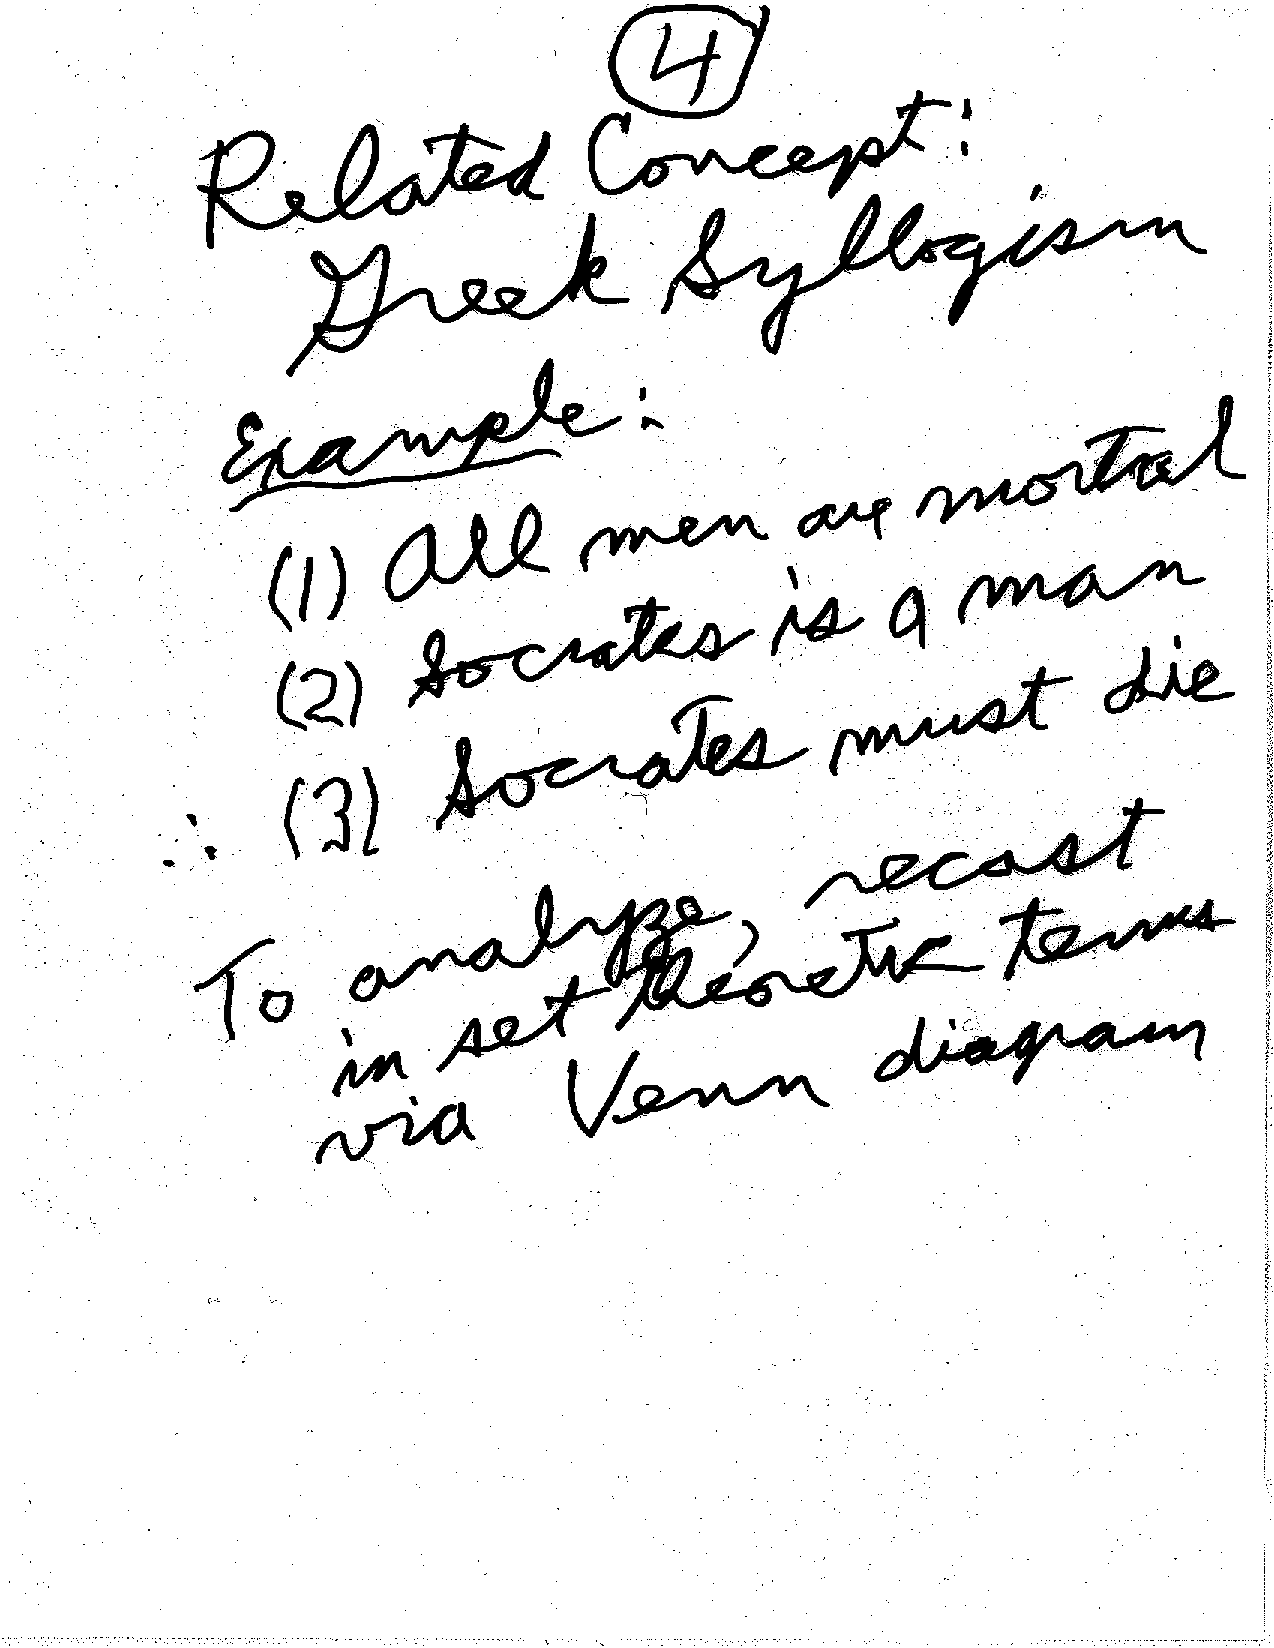
\includegraphics[scale=.5]{Pages/ST_4}

\newpage

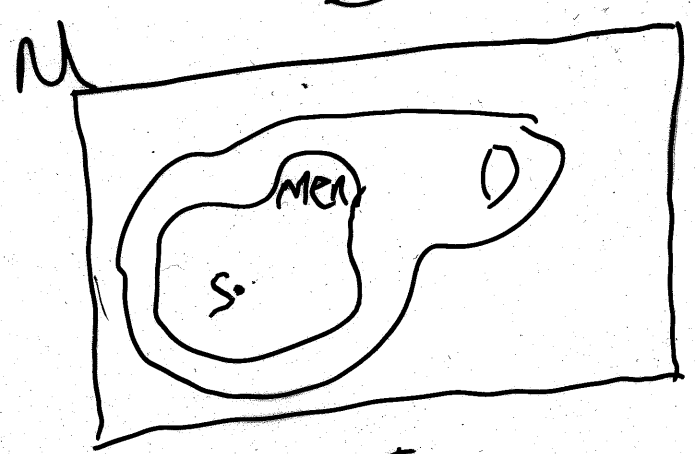
\includegraphics[scale=.2]{Pages/ST_5_im1}

$S$: Socrates\\
$M$: Set of Men\\
$D$: Things that will die\\
$\mathcal{U}$: Things on Earth

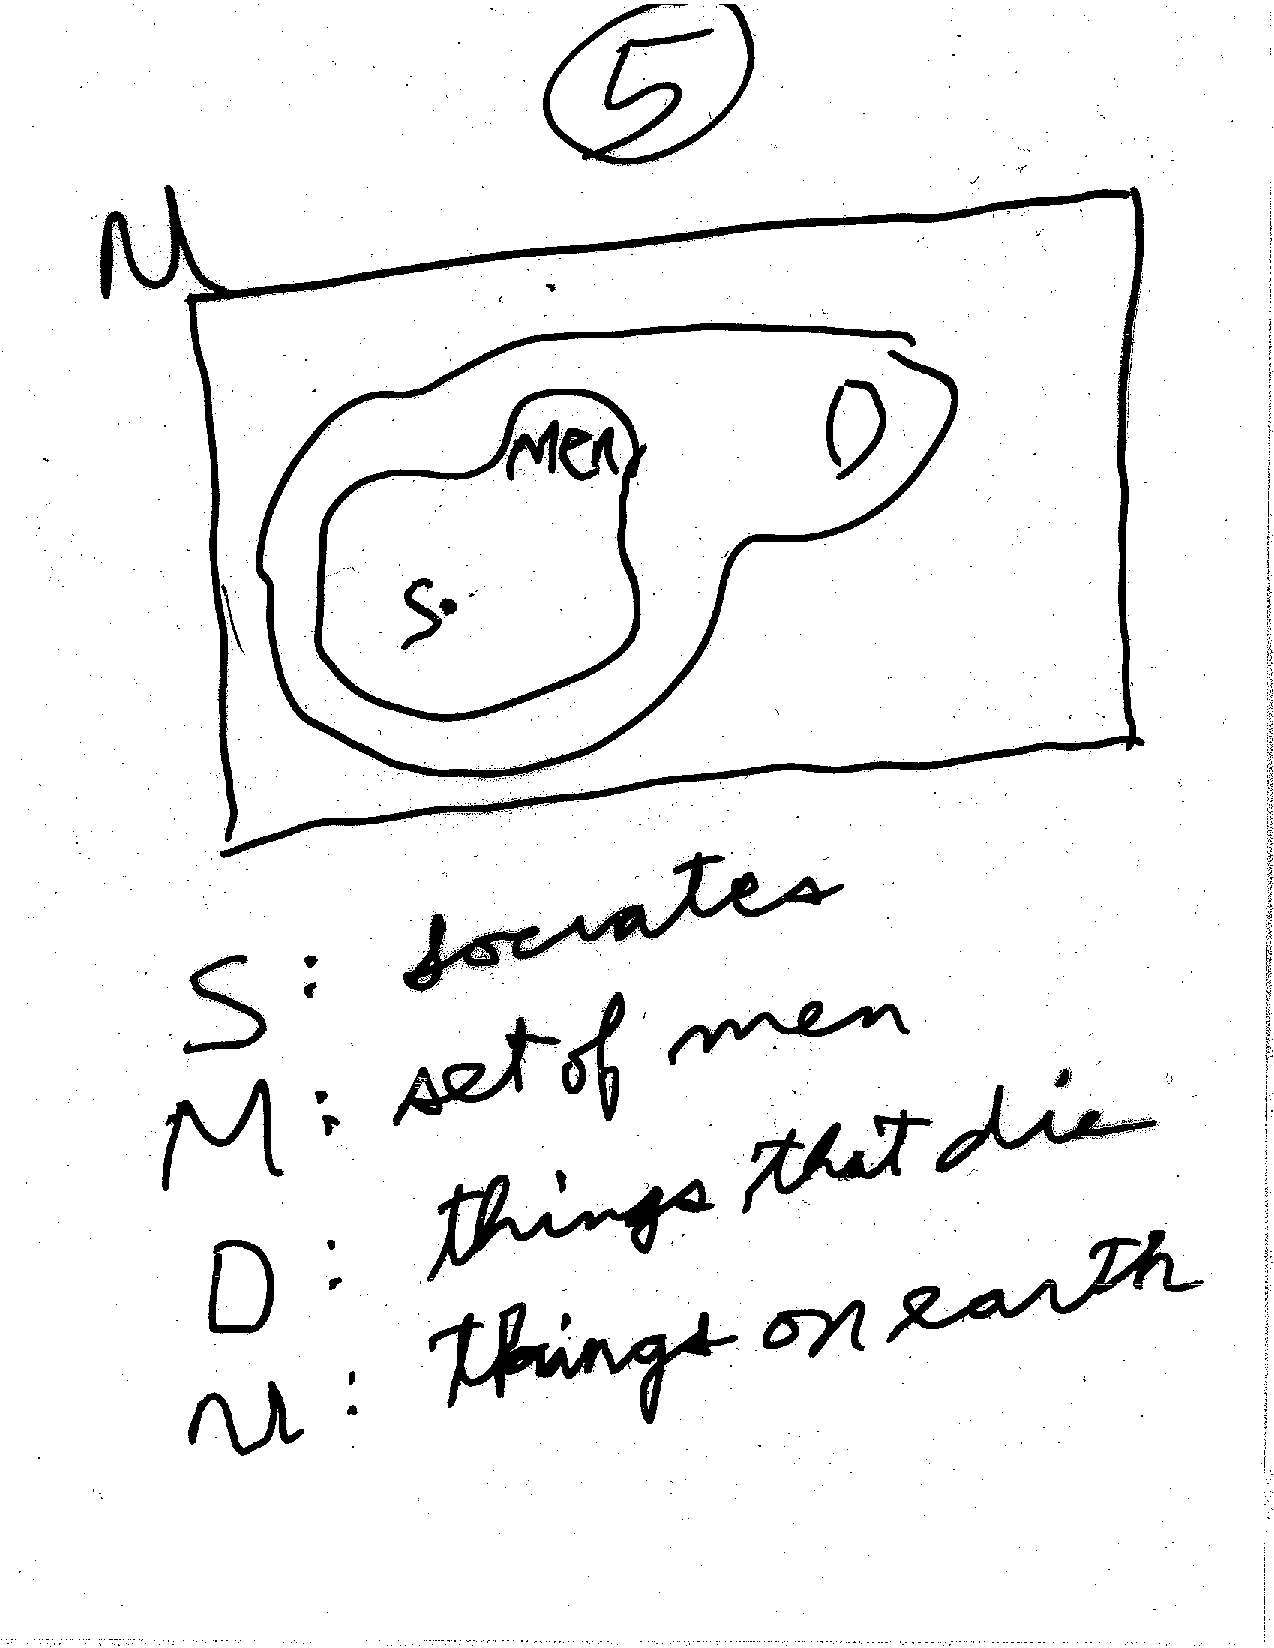
\includegraphics[scale=.5]{Pages/ST_5} 



%Zack: Pages 6,7,8,19,20

%Jack: 21, 9, 10, 11

%Koka: Pages 13, 13A, 22 ,22A, 22B


\section{Generate $\mathbb{N}$}


%Ruth: Pages L4A-L4G




\section{From $\mathbb{Z}$ to $\mathbb{R}$ via ordering}
%Jazz: ZR1-ZR5

\large
\underline{From Z to R via Orderings}\\

\normalsize

$\mathbb{Z}$ = {...,-1,0,1,...}\\We can put a strict ordering on it so that for all $n \in \mathbb{Z}$ , $n<n+1$.\\

With this ordering\\
	$0 \rightarrow 1$ in one step\\
	$0 \rightarrow 2$ in two successive step\\

Simplify for \\
	$n\rightarrow n+1$\\
	$n\rightarrow n+2$

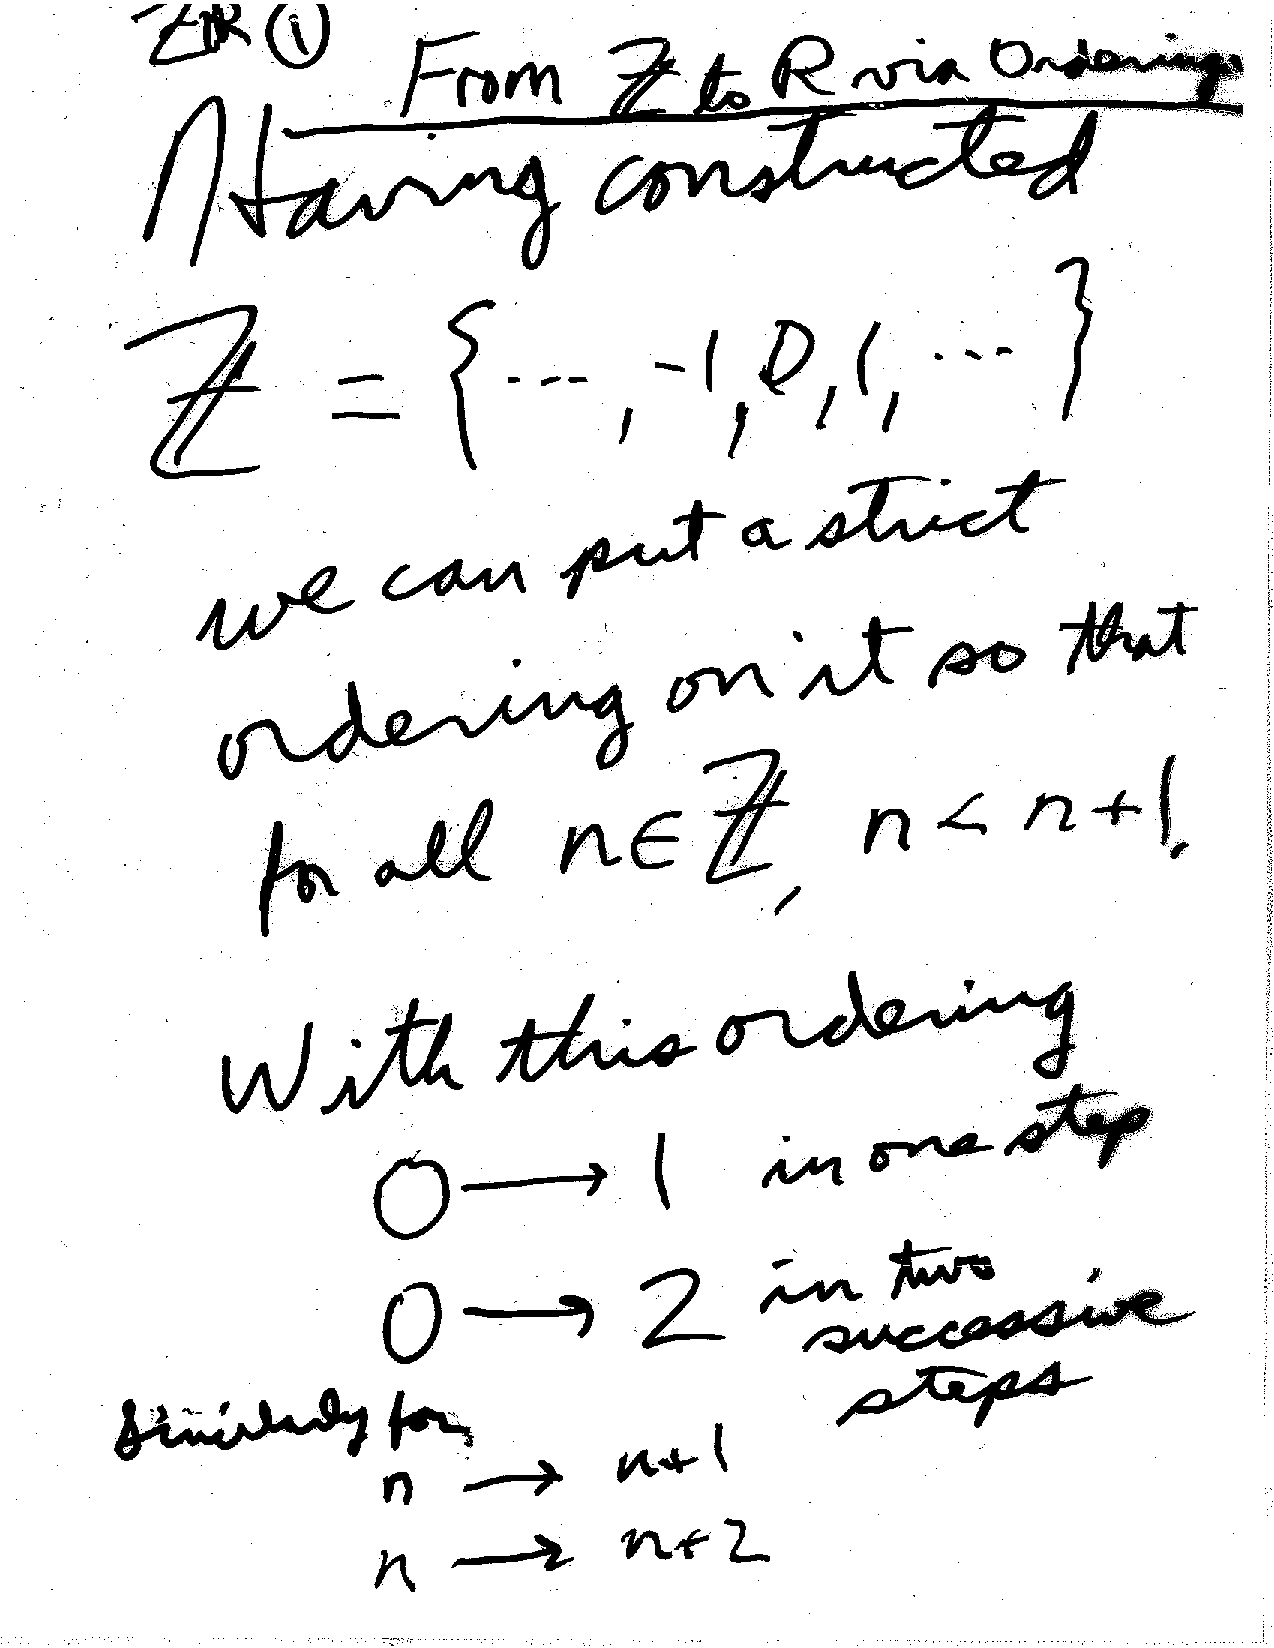
\includegraphics[scale=0.5]{Pages/ZR_1}

\newpage

Suppose we want to propose/construct the existence of a set\\
$\mathbb{Z}_{(2)}\neq \mathbb{Z}$\\
which requires two successive steps of some kind to go from\\
$0 \rightarrow 1$\\
and $n\rightarrow n+1$.\\
What is required?

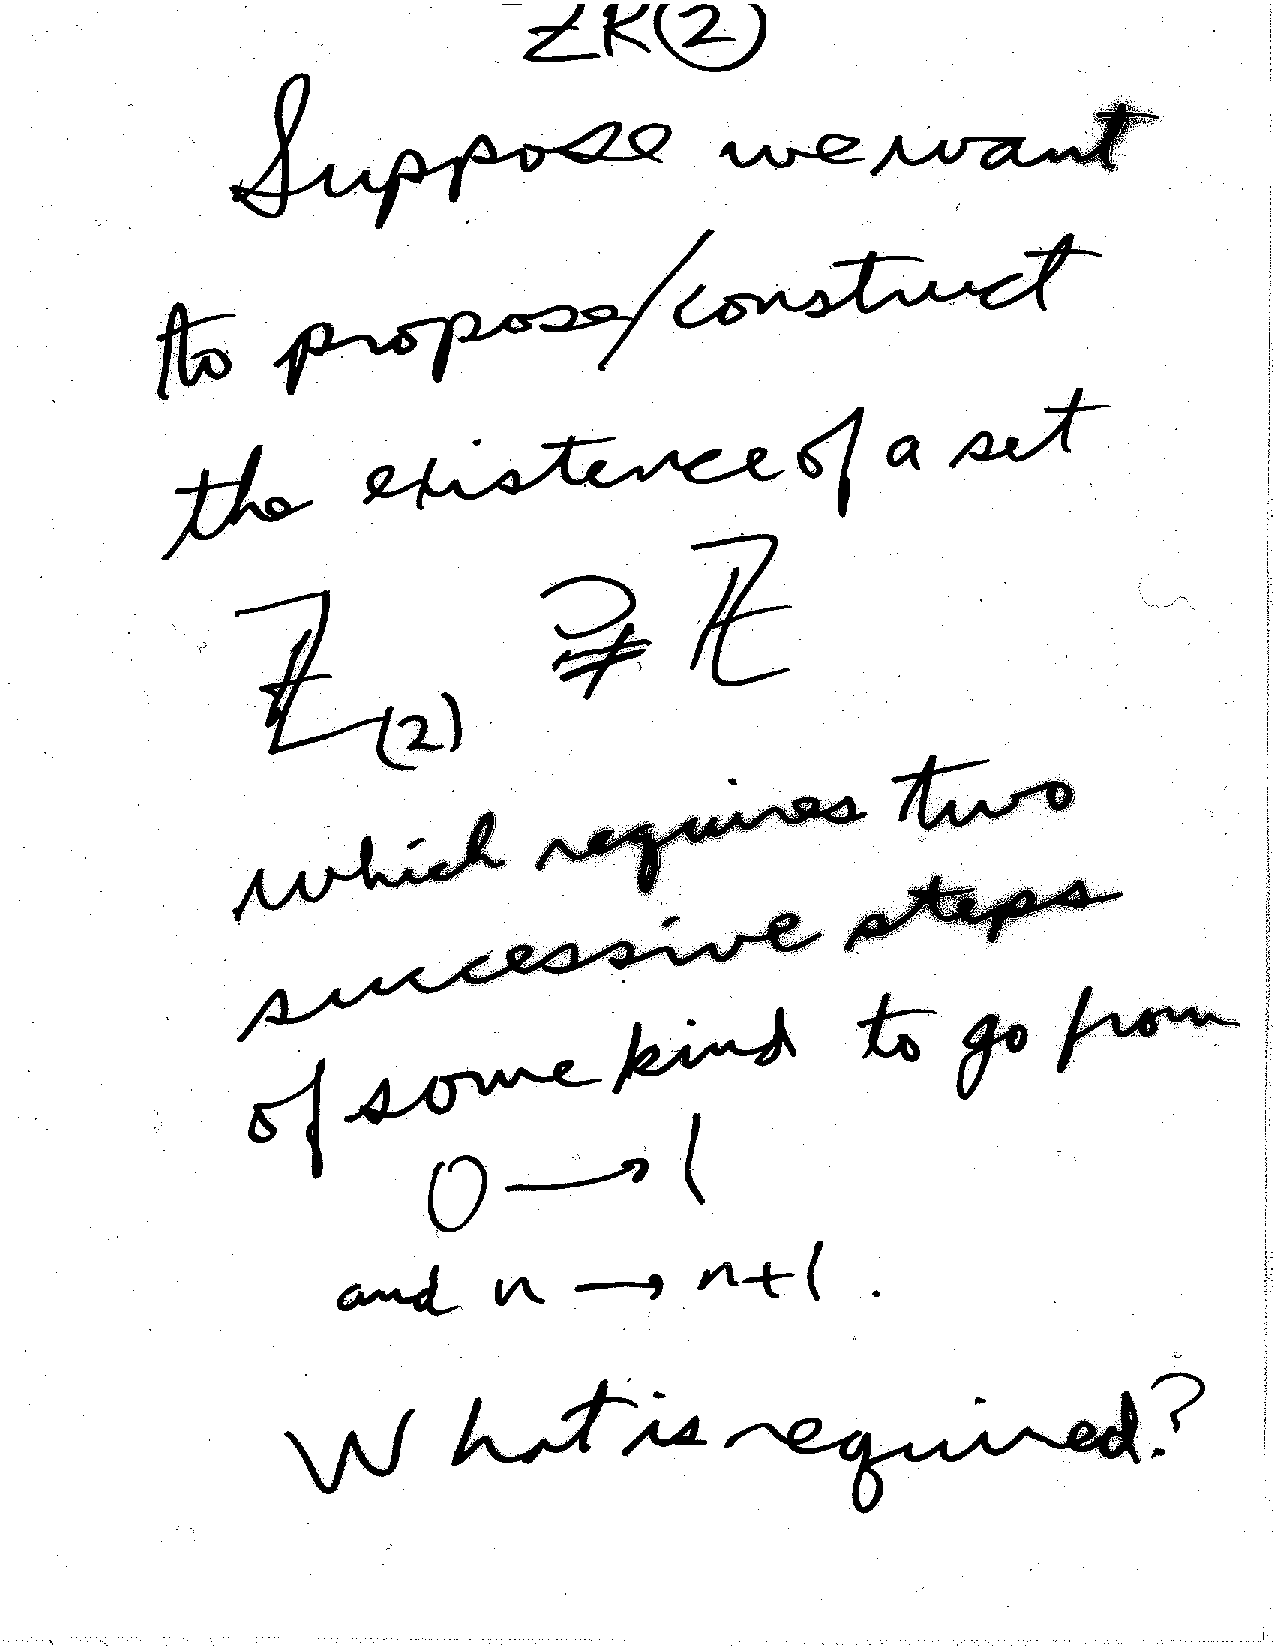
\includegraphics[scale=0.5]{Pages/ZR_2}

\newpage

We need to go from\\
$0\rightarrow x$ in one step and from $x\rightarrow1$ in the next\\
Similarly we go from $n\rightarrow n+x$ and $n+x$ to $n+1$.\\
We need a symbol to specify x. Let $x=\frac{1}{2}$.\\
Then $\mathbb{Z}_{(2)}=\mathbb{Z}\bigcup$\{$\in+\frac{1}{2}:n\in{Z}$\\
We can put an...

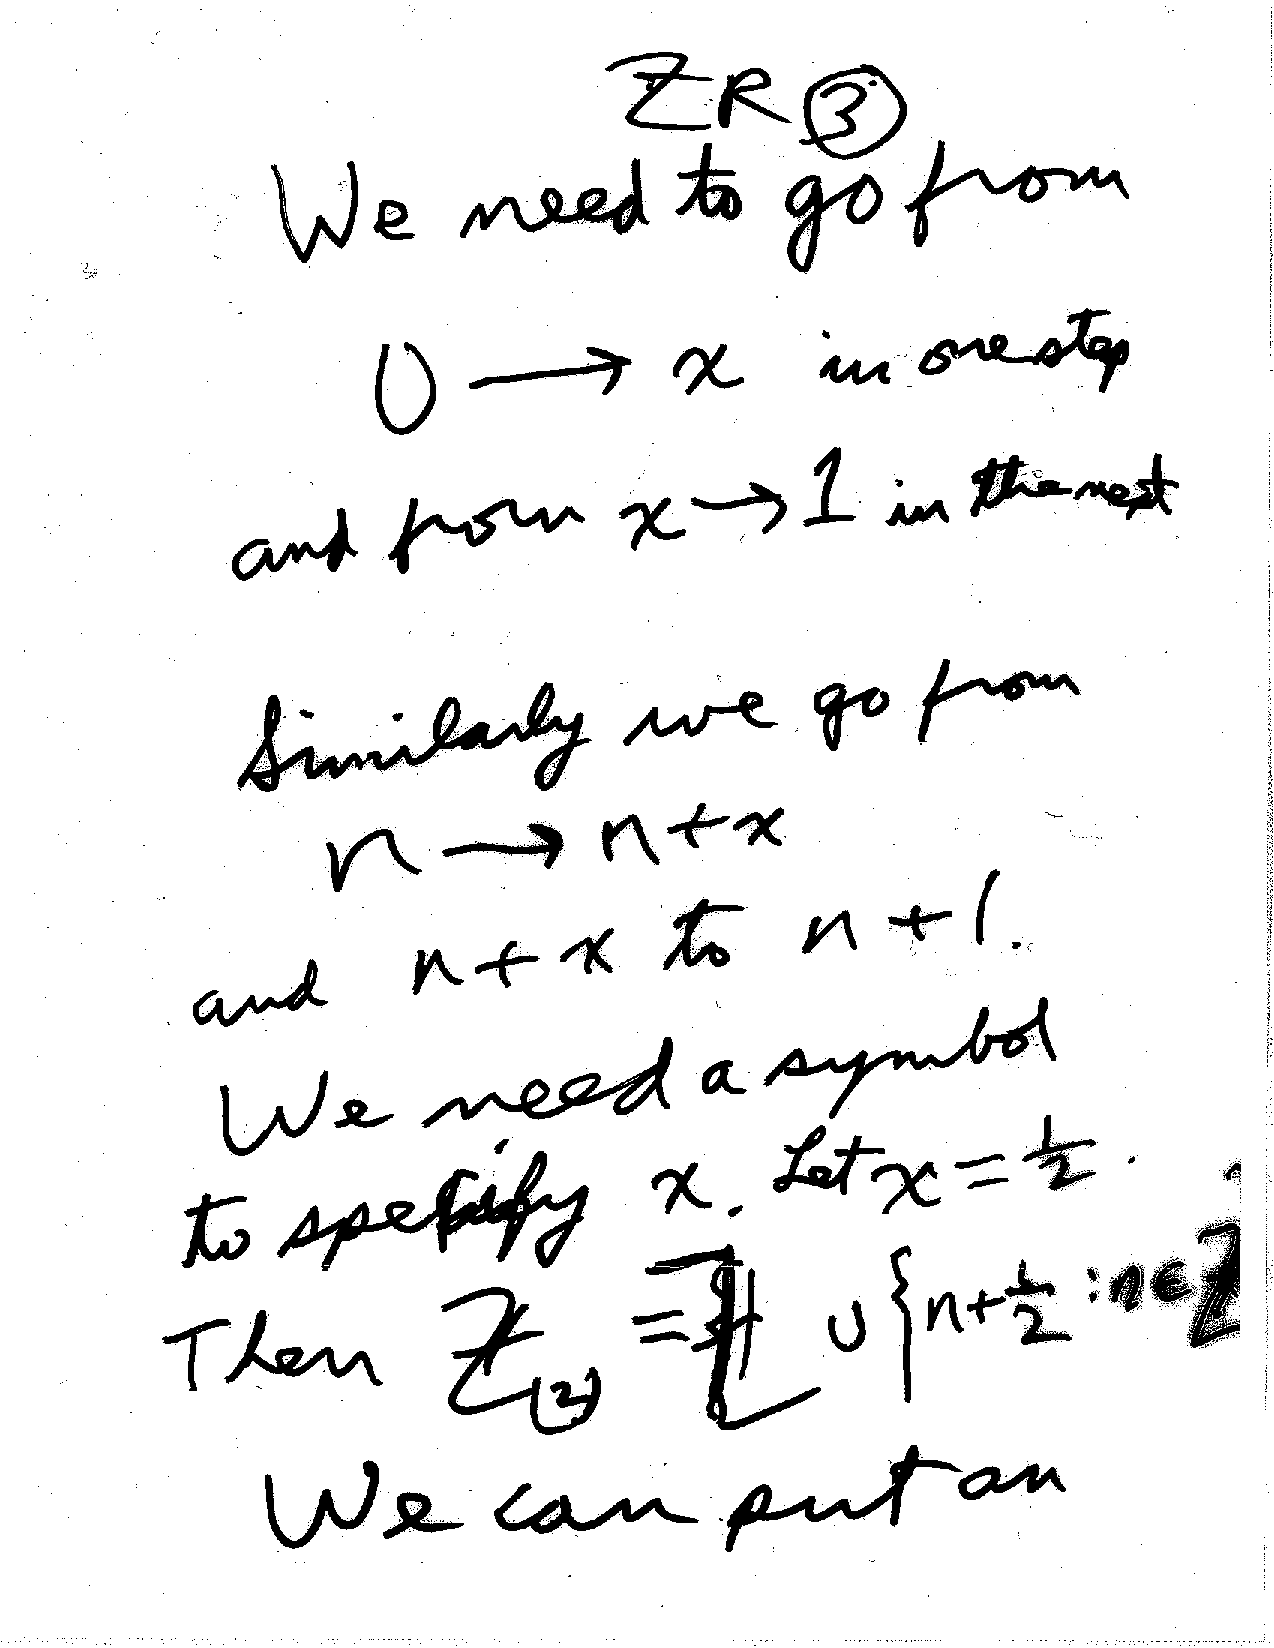
\includegraphics[scale=0.5]{Pages/ZR_3}

$\{$

\newpage

...ordering $<_{(2)}$ on $Z_{(2)}$ that \underline{extends} the ordering $<$ on $Z$. \\ 
\underline{Problem:} Let $(\mathcal{S};, <;)$ be two ordered sets such that $\mathcal{S}, \subseteq \mathcal{S}_2$.\\
\underline{Define} what it means to say that the ordering $<_{2}$ extends $<,$.\\

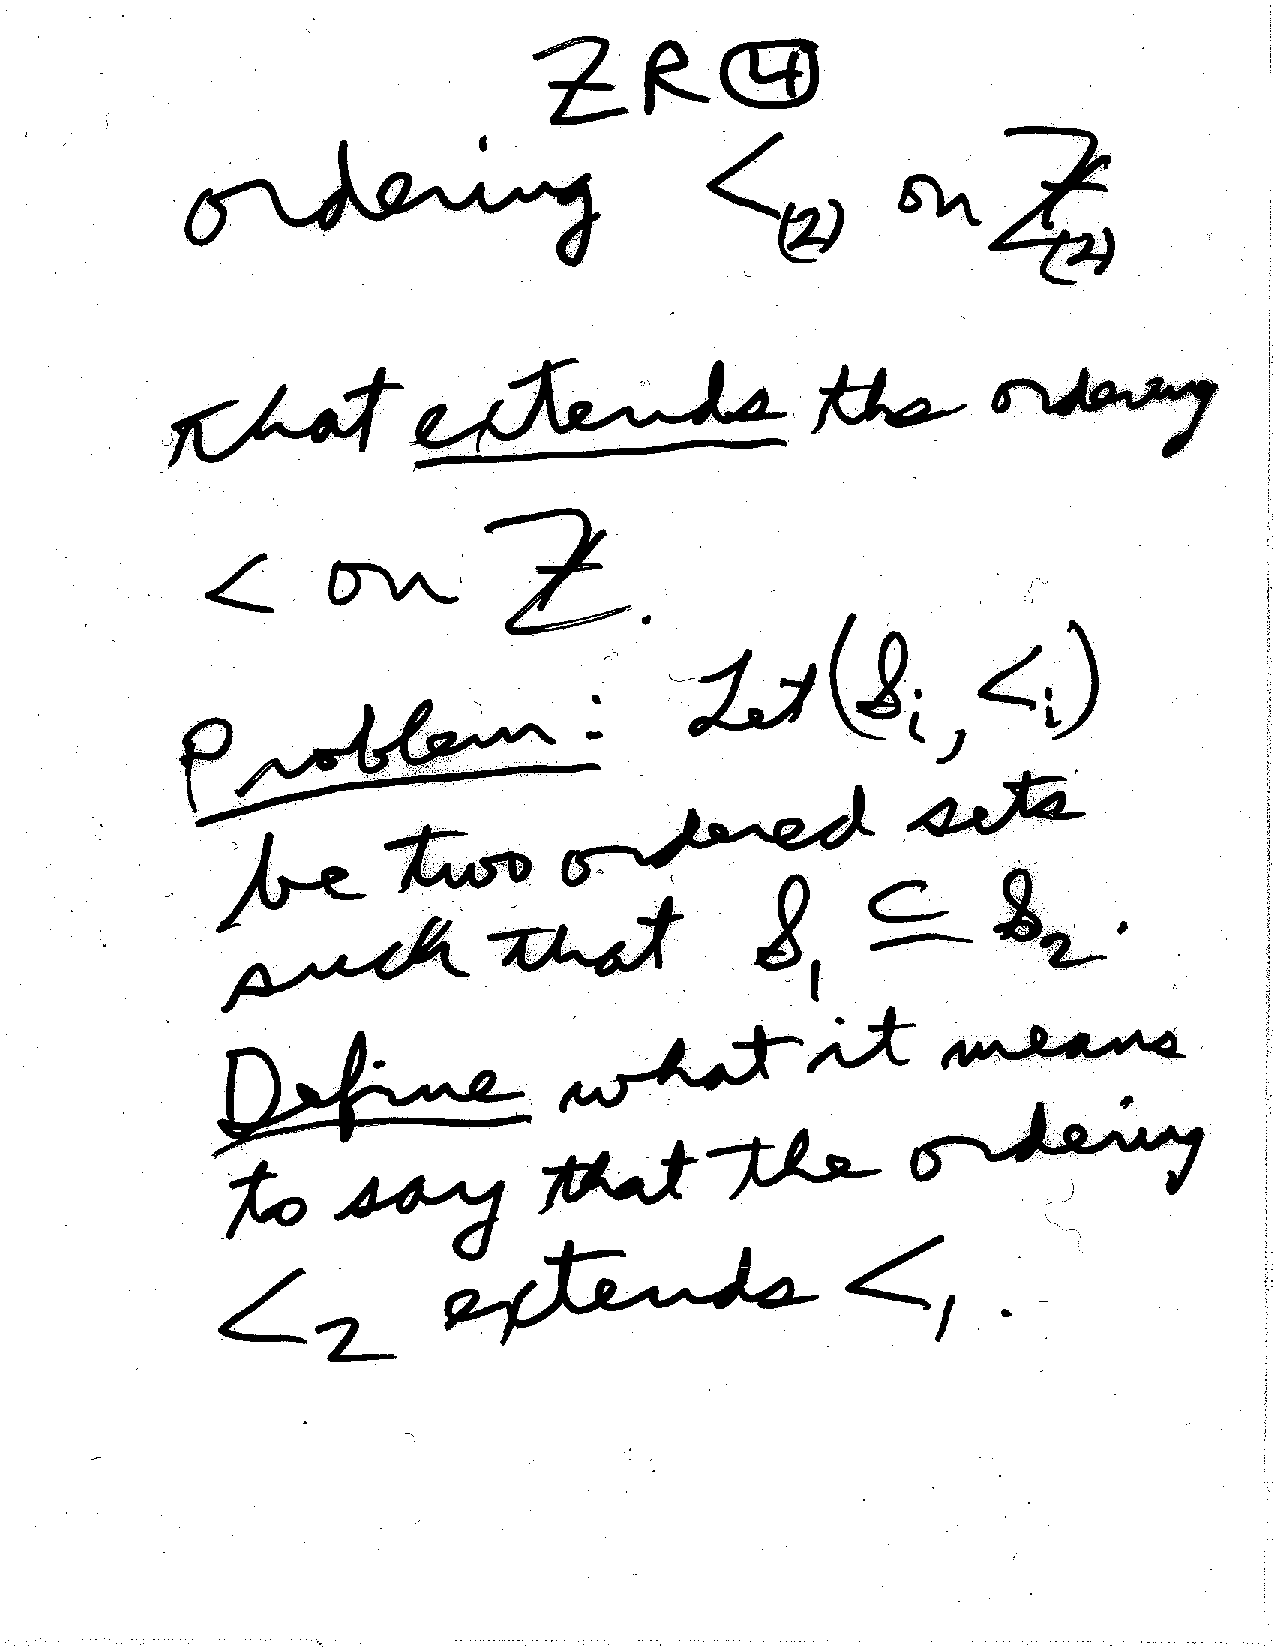
\includegraphics[scale=0.5]{Pages/ZR_4}

\newpage

For $Z_{(2)}$ there is a unique ordering $<_{(2)}$ such that\\
$n<_{(2)} n+\frac{1}{2}$ and $n+\frac{1}{2} <_{(2)} n+1$\\
Similarly, we can generate the ordered set $(Z_{(4)}, <_{4})$ where $Z_{(2)}$  sign  $Z_{(4)}$ and $<_{4}$ extends $<_{2}$

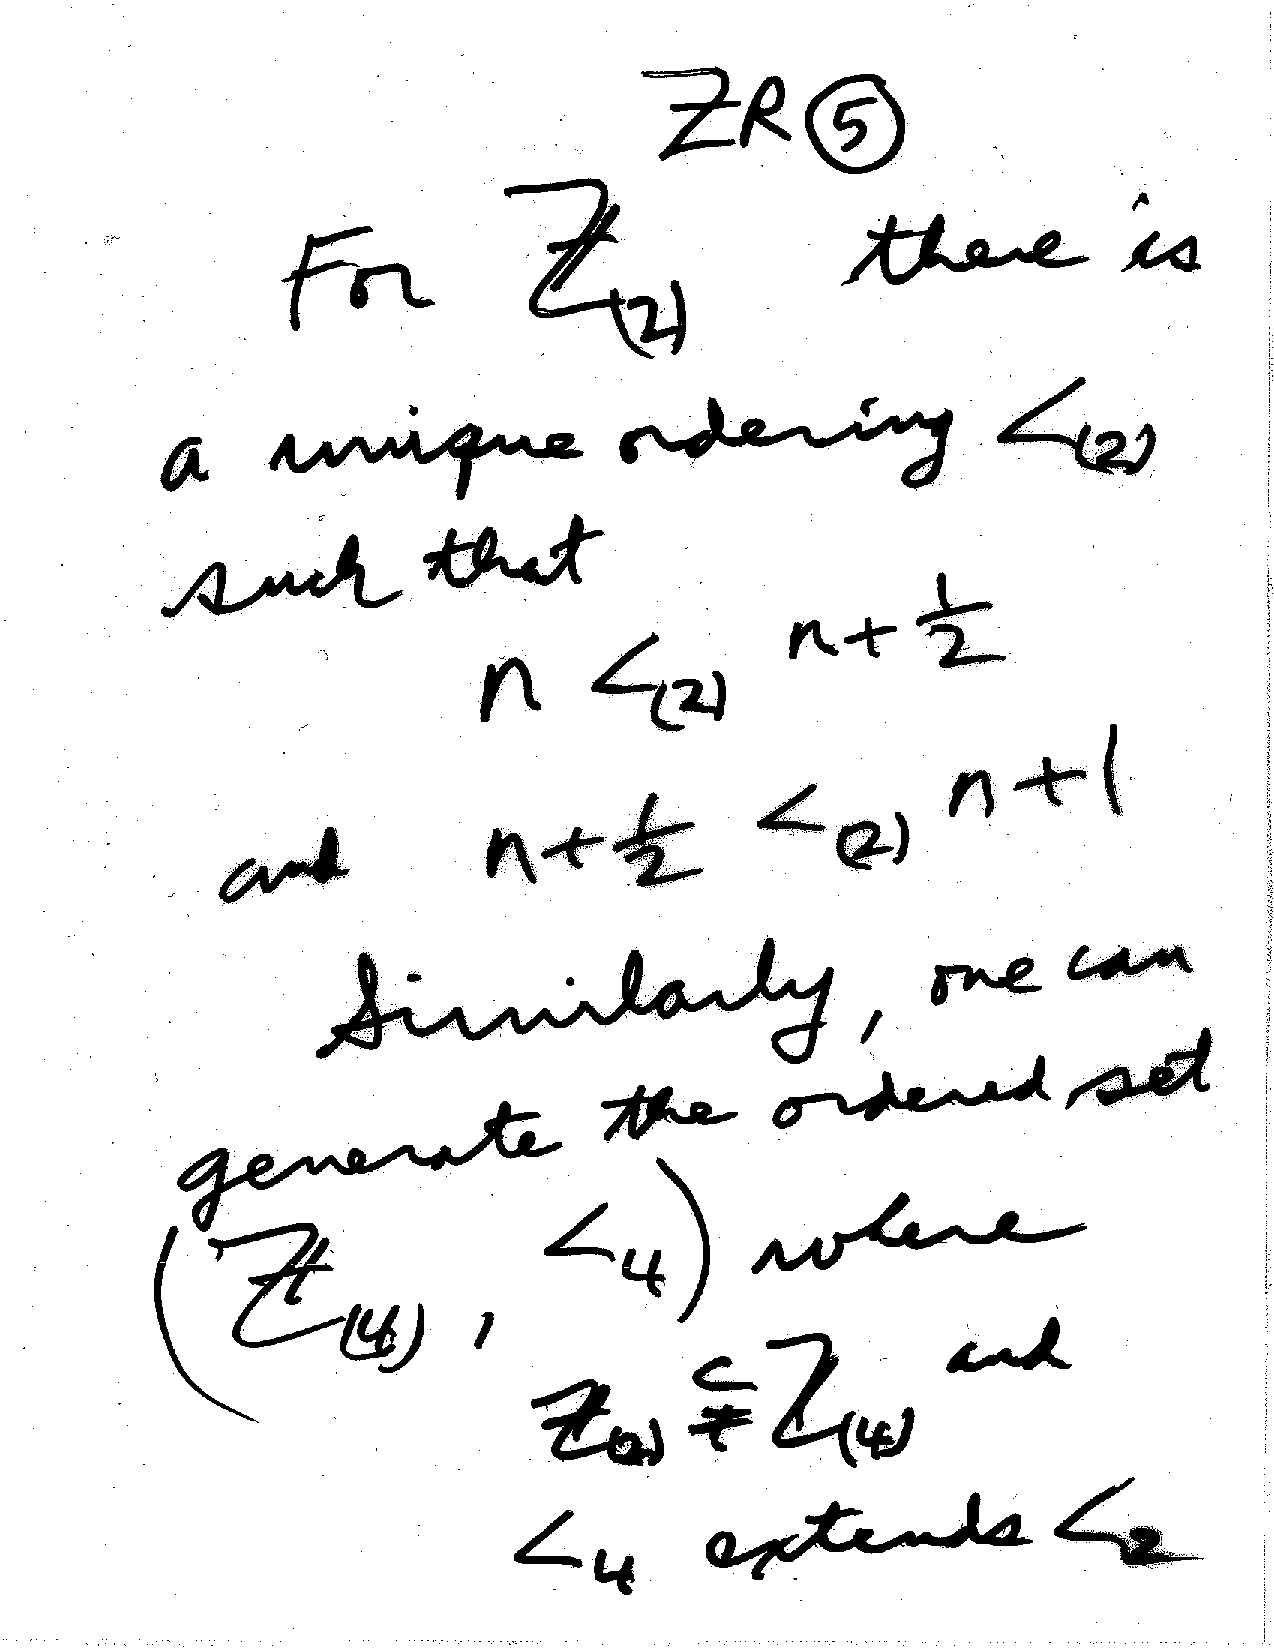
\includegraphics[scale=0.5]{Pages/ZR_5}

%Kyler: ZR6 - ZR10

%Preethika: ZR11-ZR14


\section{Sequence and Limits}

%Aaron: First 2 pages and 48-50

%Hamza: 51-52B

\section{Limit and Convergence}

%Joe: 50-51

%Quinten: 52-53

%Farishta: 53A-54A

\section{Infinite Series}

%Sukhreet: IS1 - IS 7

%Matthew: IS8 - IS15

%Will: IS16 - IS23

%Rebecca: IS24 - IS32

%Maady: IS33 - IS42

\section{Metric Spaces Part 1}

%Travis: M1 - M5

%Jerome: M6- M10



\section{Metric Spaces Part 2}


%Bryant: M1-M7

%Reshma: M8-M14

%Ethan: M15-M21





\end{document}